\scanpage{6}
\[
\begin{aligned}
(P/Q)'&=\frac{P'}{Q}-P\frac{Q'}{Q^2}=\frac{P'Q-Q'P}{Q^2}\\
(P/Q)''&=P''/Q\deleted{\unsure{+}}\unsure{-|+}2\frac{P'Q'}{Q^2}+\deleted{\unsure{2}}P\bigl(
\end{aligned}
\]
\[
\frac{P'}{\deleted{Q}P}-\frac{Q'}{Q}
\]
\[
(xy)^{\unsure{2|''}}=\unsure{x''|x^2}y+2x'y^{\unsure{\prime}}+xy^{\unsure{\prime\prime|\prime}}
\]
\[
\left(\frac{\deleted{\unsure{P'}}f}{g}\right)'=\frac{f'g-g'f}{g^2}
\]
\[
\frac{(P''Q+\deleted{P'Q'}-\deleted{P'Q'}\deleted{\unsure{+}}\unsure{-|+}Q''P)Q^{\unsure{\deleted{2}|2}}
 -(P'Q-Q'P)2\deleted{Q}Q'}{Q^3}
\]
% The second fraction rule follows the separate lower tracing beneath the right-middle part.
\figure{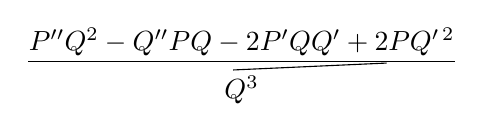
\begin{tikzpicture}
\node[inner sep=0pt,anchor=south west] (num) at (0,0)
 {$P''Q^2-Q''PQ-\unsure{2}P'QQ'+2PQ'^{\,2}$};
\path (num.south west)--(num.south east) coordinate[pos=0.48] (partialstart);
\path (num.south west)--(num.south east) coordinate[pos=0.84] (partialend);
\draw ([yshift=-2pt]num.south west)--([yshift=-2pt]num.south east);
\draw ([yshift=-5pt]partialstart)--([yshift=-2.5pt]partialend);
\node[inner sep=0pt,anchor=north,yshift=-7pt] at (num.south) {$Q^3$};
\end{tikzpicture}}
% The small quotient's fraction rule turns back at its right end; no arrow meaning is assigned.
\figure{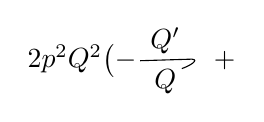
\begin{tikzpicture}
\node[inner sep=0pt,anchor=base west] (prefix) at (0,0) {$2p^2Q^2\bigl(-$};
\node[inner sep=0pt,anchor=south] at ([xshift=0.36cm,yshift=0.08cm]prefix.east) {$Q'$};
\node[inner sep=0pt,anchor=north] at ([xshift=0.36cm,yshift=-0.10cm]prefix.east) {$Q$};
\draw ([xshift=0.04cm]prefix.east)--([xshift=0.70cm,yshift=0.02cm]prefix.east)
 .. controls ([xshift=0.80cm,yshift=0.01cm]prefix.east) and ([xshift=0.66cm,yshift=-0.07cm]prefix.east)
 .. ([xshift=0.57cm,yshift=-0.10cm]prefix.east);
\node[inner sep=0pt,anchor=west] at ([xshift=0.97cm]prefix.east) {$+$};
\end{tikzpicture}}

% Opposite-direction writing, read after a half-turn. Two long diagonals cancel this layer.
\[
\deleted{\det\begin{pmatrix}a\deleted{\unsure{d|b}}&c\\b&d\end{pmatrix}-ad-bc\quad\text{inversible}}
\]
\[
\deleted{\begin{array}{c@{}l}
\delta(e_1 e_{d-2})&=-e_1\delta(e_{d-2})=-e_1e_{d-3}\deleted{=e_d}\\
\rotatebox{90}{$=$}&\\
\delta(a\eta)&=a\delta\eta=a\alpha e_{d-2}+a\beta f_{d-2}
\end{array}}
\]
\[
\deleted{\begin{array}{c@{}l}
\delta(e_1 f_{d-2})&=-\deleted{f}e_1\cdot f_{d-3}\\
\rotatebox{90}{$=$}&\\
b\alpha e_{d-2}+b\beta f_{d-2}&
\end{array}}
\]
\[
\deleted{\begin{array}{c@{}l}
\delta(f_1 e_{d-2})&=\delta(f_1)e_{d-2}-f_1\delta(e_{d-2})=e_{d-2}-f_1e_{d-3}\\
\rotatebox{90}{$=$}&\\
\delta(c\eta)&=c\delta\eta=c\alpha e_{d-2}+c\beta f_{d-2}
\end{array}}
\]
\deleted{etc}

% Detached dot at full-scan x=965--973, y=598--607, below and left of On after rotation.
% Its hand, layer, role, and cancellation state are unresolved; no relation to the formula is assigned.
\(\underset{\unsure{\text{.}}}{\phantom{\text{On}}}\)\deleted{On en tire $e_1e_{d-3}$, $\deleted{f}e_1f_{d-3}$\unsure{,} $f_1e_{d-3}$, $f_1f_{d-3}$ comme comb. lin des $e_{d-1}$ et $f_{d-2}$, à coeff entiers fonctions de $\alpha,\beta$, $a,b,c,d$}

\[
\deleted{\begin{array}{c@{}l}
\delta(e_1x_i)&=-e_1\delta(x_i)=-e_1\deleted{\unsure{\delta}}x_{i-1}\qquad 2\leq i\leq{}\\
\rotatebox{90}{$=$}&\\
\delta(\deleted{\unsure{S}}s e_{i+1}+t f_{i+1})&=s e_i+t f_i
\end{array}}
\]
% archive sheet number: 5
